\section{Mixer}

\subsection{ADL5802}
\label{sec:adl5802}


The mixer schematic shown in Figure~\ref{fig:mixer-sch} is composed of three high-frequency baluns
that convert two rx and one local oscillator (the original transmitted signal) single-ended signal
into differential signals and then feed them into the mixer. The baluns are
\href{https://www.johansontechnology.com/datasheets/baluns/Balun_5400BL15B050.pdf}{5400BL15B050E}
and the mixer is
\href{http://www.analog.com/media/en/technical_documentation/data_sheets/ADL5802.pdf}{ADL5802}. The
mixer outputs the difference of the local oscillator frequency and each R input which ranges from
hundreds of kHz to a few MHz.

\begin{figure}[ht]
  \centering
  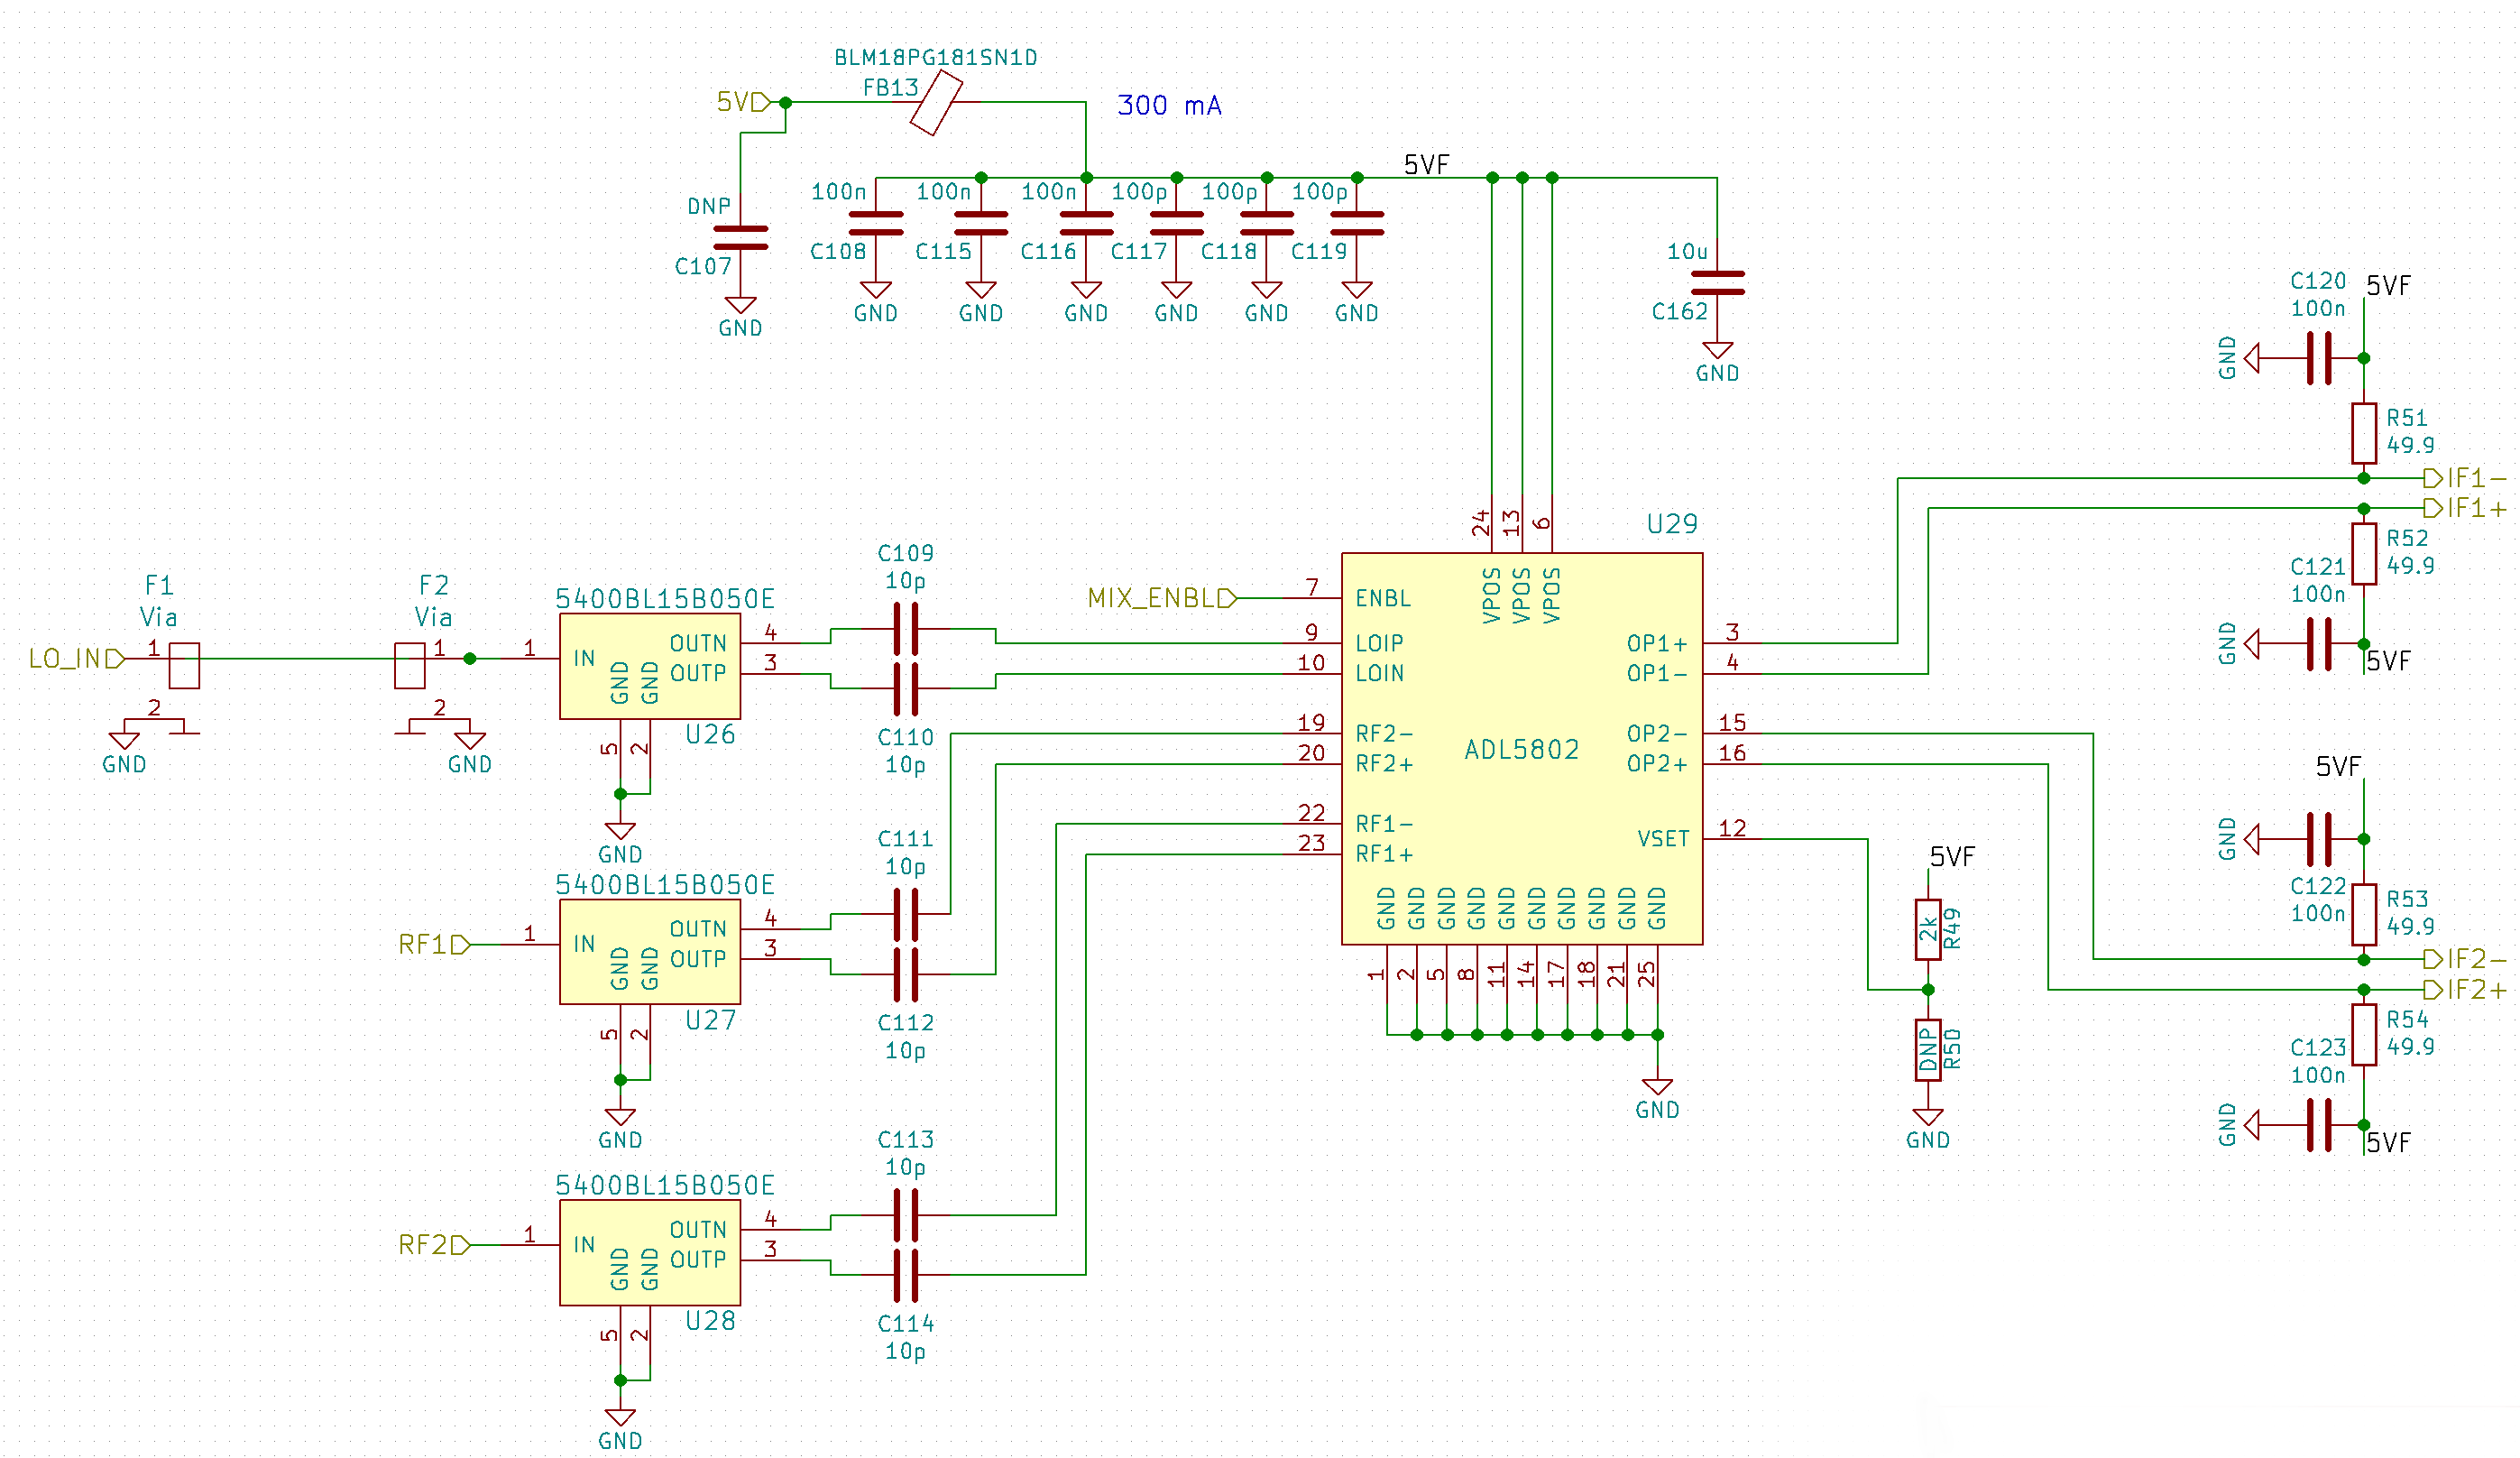
\includegraphics[width=\textwidth]{data/mixer-sch.png}
  \caption{The mixer schematic.}
  \label{fig:mixer-sch}
\end{figure}

The RF and LO input interfaces are designed for a differential input impedance of 50$\Omega$. This
is already the differential balanced impedance of the baluns, so we do not need to perform any
additional impedance matching at the inputs. The inputs require AC coupling and the datasheet
recommends 3pF coupling capacitors placed between the balun outputs and pin inputs. It also shows
that the positive balun output of the local oscillator should be hooked up to the positive pin
input.